\subsection{建造者模式(Builder)}

\subsubsection{建造者模式简介}

建造者模式是一种创建型设计模式,它提供了一种将一个复杂对象的构建与它的表示分离的方式,通过定义一个建造者来构建复杂对象的不同部分,最终构建出完整的复杂对象。

建造者模式包括如下角色:

建造者(Builder):定义构建复杂对象的接口,包括构建复杂对象的各个部分的操作。
具体建造者(Concrete Builder):实现建造者接口,完成构建复杂对象的各个部分的操作。
指挥者(Director):负责构建复杂对象,通过调用建造者接口中的方法来构建复杂对象的各个部分。
产品(Product):表示复杂对象,包含多个组成部分。

通常,建造者模式适用于以下场景:

在创建一个复杂对象的同时,需要指定其各个部分的构建顺序。
创建复杂对象的算法应该独立于该对象的组成部分以及它们的装配方式。
在创建复杂对象时,提供一个高层接口来指定各个部分的装配方式,并不暴露该对象的内部组成部分。
建造者模式提供了一种将复杂对象的构建与它的表示分离的方式,可以使得客户端不必知道复杂对象的具体构建细节,且可以更加精细地控制复杂对象的构建过程。

\subsubsection{建造者模式在项目中的应用}

\begin{figure}[htb]
  \centering
  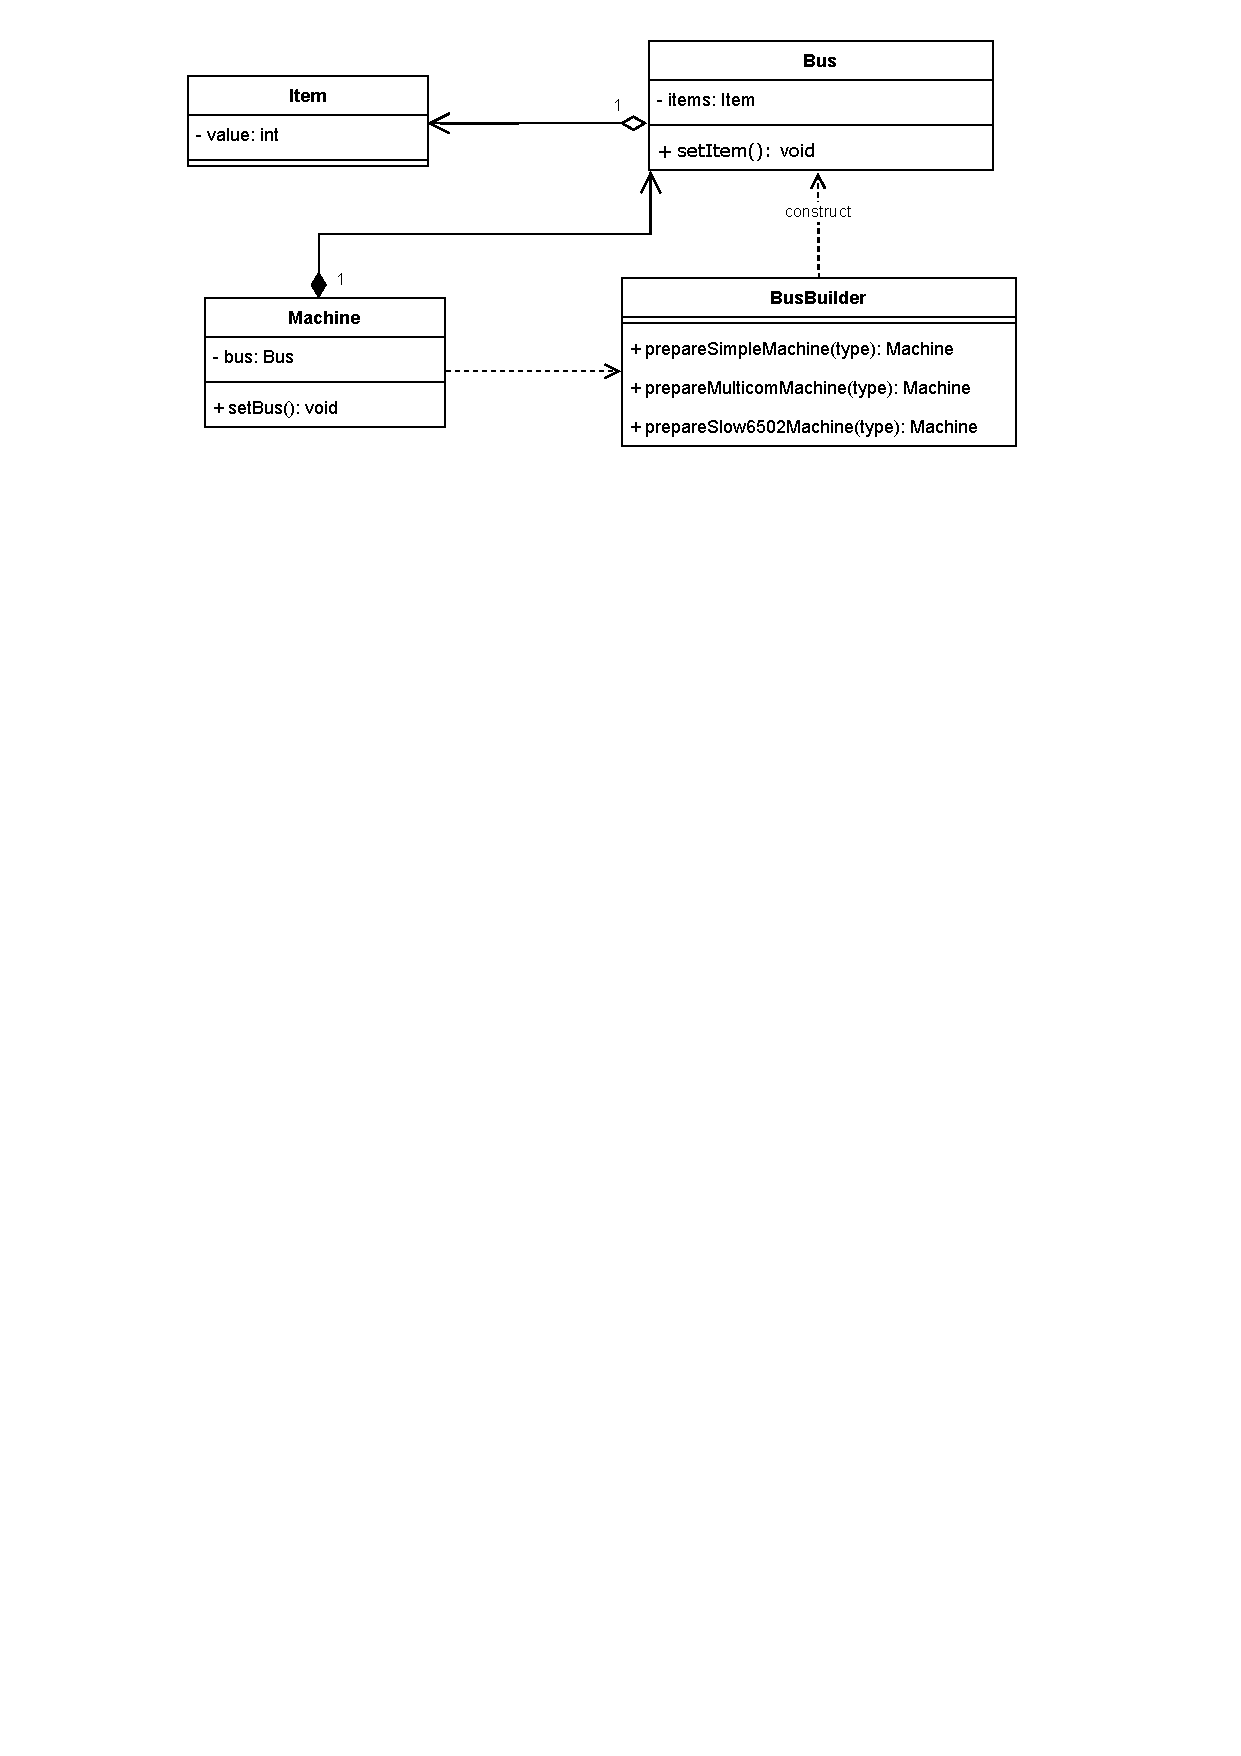
\includegraphics[width=0.9\textwidth]{figures/建造者.pdf}
  \caption{建造者模式在 Slow6502 中的类图}
\end{figure}

项目中Bus的构建使用了建造者模式,在不同的Machine里面可以使用不同的组装方法来构造出不同的 Bus,并且可以在不同的 Machine 中使用。这样,在不同的 Machine 中,就可以使用适当的组装方法来构造出最合适的 Bus,从而提高系统的灵活性和可扩展性。

另外,使用建造者模式还可以使得在构建 Bus 时分离具体的构造过程和最终的产品。这样,可以在不影响最终的产品的情况下,修改或替换构造过程中的某些步骤,这有助于提高项目的可维护性和可扩展性。
